\chapter{Verwandte Arbeiten}
\label{chap:relwork}
 \phantom{Liste Bücher die nicht zitiert werden: \cite{RTR3}\cite{gpugems1}\cite{gpugems2}\cite{gpugems3}\cite{cgtutorial}}
An dieser Stelle werden einige Veröffentlichungen vorgestellt, die sich mit ähnlichen Problemstellungen befassen, wie die vorliegende Arbeit.
\todo[size=\small, color=yellow!40, inline]{Kapitel: Human proofreading}%
Das $c$-Collision Protokoll \cite{ccol3} ist ein Protokoll welches eine möglichst gleichförmige Verteilung von Aufgaben auf eine begrenzte Anzahl von Ressourcen zu erreichen versucht. $c$ ist eine Konstante. Erhält eine Ressource höchstens $c$ Anfragen, werden alle beantwortet. Sind es mehr, werden keine beantwortet. Durch das konstante $c$ kann es passieren, dass nicht alle Aufgaben verteilt werden können. Mit einer Modifikation des Protokolls können solche Verklemmungen vermieden werden. Dabei werden mehrere Runden abgearbeitet. Sollten in einer Runde keine weiteren offenen Aufträge vergeben werden, wird $c$ erhöht. Es gibt also irgendein $c$, für das das Protokoll terminiert. Die Effizienz des Protokolls lässt sich noch steigern, wenn die Ressourcen zufällig und redundant verteilt werden \cite{ccol4}.

In der Arbeit von Berenbrink et al. \cite{ccol2} wird das $c$-Collision Protokoll von Stemann \cite{ccol3} modifiziert, um mit gewichteten Aufgaben arbeiten zu können. Ausgehend von $m$ Bällen, welche auf $n$ Körbe verteilt werden, wird eine untere Schranke für $m \ge n$ ermittelt, in Abhängigkeit der Runden und Anzahl der Körbe. Außerdem wird ein Zusammenhang zwischen der Anzahl der Bälle, der Gleichförmigkeit ihrer Gewichte, sowie der benötigten Laufzeit zur Erreichung einer gegebenen Last, untersucht. In dem Algorithmus, dem "`$c$-Load Collision Protocol"', wählt jeder Ball zufällig drei Körbe. Es werden mehrere Runden durchgeführt. In jeder Runde stellt jeder Ball eine Anfrage samt seines Gewichts an alle gewählten Körbe. Jeder Korb berechnet die Summe aller Gewichte von allen Anfragen an ihn. Ist diese Summe höchstens $c$, akzeptiert er, sonst lehnt er ab. Hat ein Ball mindestens eine akzeptierende Antwort bekommen, wird er, samt der durch ihn gestellten Anfragen, aus dem Protokoll entfernt.\\
Dieser Algorithmus ist genau der, der auch in der vorliegenden Arbeit benutzt wird (siehe \ref{sec:basics:algos}).
\section{Paralleles Rendering}
\label{sec:relwork:parrender}
Beim parallelen Rendering geht es um digitale Bilderzeugung durch parallele Aufgabenverteilung. Eine populäre Möglichkeit für paralleles Rendering bietet das Scalable Link Interface (SLI), bei dem mehrere Grafikprozessoren zusammen geschlossen werden, um eine höhere Leistung zu erzielen. Es ist aber auch möglich parallel innerhalb eines Netzwerks im Rechnerverbund (Cluster) zu rendern. Dabei wird meist das Rendern selbst in verschiedene Unteraufgaben geteilt. Eine weitere Möglichkeit parallel zu rendern ist die Trennung von Aufgaben, die im Eigentlichen nichts miteinander zu tun haben, wie zum Beispiel eine Trennung der Datenverwaltung von der Bilderzeugung.\\
In den letzten Jahren wurden viele Möglichkeiten zur Verteilung der Aufgaben in parallelen Rendersystemen veröffentlicht. Molnar et al. \cite{molnar} klassifizieren Parallelisierungsstrategien in drei Kategorien, die sich durch die Stelle innerhalb der Rendering-Pipeline unterscheiden, in der die Polygone nach ihrer Sichtbarkeit sortiert werden. Diese drei Klassifizierungen werden Sort-First, Sort-Midlle und Sort-Last genannt.

Sort-First-Algorithmen teilen den Bildschirm in Regionen ein (Kacheln) und weisen jedem Renderer eine solche Kachel zu. Jeder Renderer ist für die gesamte Bilderzeugung in diesem einem Bildabschnitt zuständig. Geometrische Objekte werden zu den Renderern übertragen, wenn diese in der jeweiligen Kachel sichtbar sind. Sort-First-Renderer nutzen die Frame-to-Frame-Kohärenz gut aus, da typischerweise nur wenige geometrische Primitive\footnote{Geometrische Primitive sind einfache 3-D- (z.B. Kugel, Kegel, Quader, Zylinder, Torus) oder 2-D-Grundkörper (z.B. Linie, Kreis, Rechteck, Vieleck, Stern), deren Größe und Grundform über Parameter gesteuert werden können. \cite{medieninfo}} zwischen einzelnen Frames die Bildausschnitte wechseln (Abbildung \ref{fig:relwork:sortfirst}). Die Rendering-Algorithmen sind bei Sort-First frei wählbar, da jeder Renderer die vollständige Geometrie für seine Kachel besitzen muss. Allerdings kann es sein, dass sich viele geometrische Objekte der gesamten Szene auf wenige Kacheln verteilen, wodurch die Lastverteilung aus dem Gleichgewicht gerät. Da jeder Renderer sämtliche Geometrie innerhalb seiner Kachel zeichnet, werden Objekte redundant bearbeitet, wenn diese von inneren Kachelkanten geschnitten werden.
\begin{figure}
 \centering
  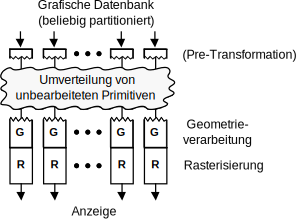
\includegraphics[scale=0.8]{images/sort-first.pdf}
  \caption{Sort-First. Umverteilung von unverarbeiteten Primitiven während der Geometrieverarbeitung. \textit{Quelle: nach \cite{molnar}}}
 \label{fig:relwork:sortfirst}
\end{figure}

Sort-Middle-Algorithmen verteilen hingegen Primitive mitten in der Rendering-Pipeline. Die Trennung erfolgt zwischen der Geometrieverarbeitung und der Rasterisierung. Vor der Verteilung werden die Objekte in screen-space Koordinaten überführt. Geometrieprozessoren bekommen eine beliebige Untermenge an Primitiven zugewiesen. Rasterisierer bekommen einen Teil des finalen Bildes zugewiesen, ähnlich wie beim Sort-First-Ansatz. Ob diese beiden Prozessortypen baulich getrennt sind, oder sich einen physikalischen Prozessor teilen, spielt dabei keine Rolle. In der Geometriestufe wird jedes Objekt bezüglich seiner finalen Bildposition klassifiziert und anschließend an die zuständigen Rasterisierer übermittelt (Abbildung \ref{fig:relwork:sortmiddle}). Ein großes Problem bei diesem Verfahren stellt jedoch die Unterbrechung der Rendering-Pipeline dar. In aktuellen Consumer-Grafikkarten ist es entweder sehr teuer, die Pipeline zu unterbrechen, oder es ist überhaupt nicht möglich. Die GPU müsste dafür mit der CPU synchronisiert werden, welches Zeit kostet und zulasten der Bildrate geht.
\begin{figure}
 \centering
  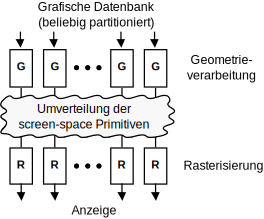
\includegraphics[scale=0.8]{images/sort-middle.pdf}
  \caption{Sort-Middle. Umverteilung von screen-space Primitiven zwischen Geometrieverarbeitung und Rasterisierung. \textit{Quelle: nach \cite{molnar}}}
 \label{fig:relwork:sortmiddle}
\end{figure}

Sort-Last-Algorithmen verteilen geometrische Objekte an einzelne Renderer. Ein Renderer berechnet Pixelwerte für seine Untermenge an Objekten und verteilt die Farb- und Tiefenwerte an Prozesse, die diese dann vereinigen (Abbildung \ref{fig:relwork:sortlast}). Bei großen Objektmengen bietet sich dieses Verfahren an, da jedes geometrische Objekt genau einmal gerendert wird. Für den Pixeltransfer wird allerdings eine hohe Bandbreite im Netzwerk benötigt. Da die genaue Tiefe eines Pixels erst bei der Vereinigung der Pixel ermittelt werden kann, ist Sort-Last für einige Rendertechniken, wie Transparenz oder Antialiasing, schlecht geeignet.
\begin{figure}
 \centering
  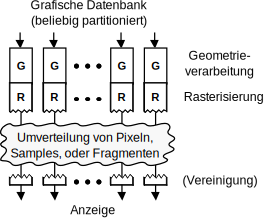
\includegraphics[scale=0.8]{images/sort-last.pdf}
  \caption{Sort-Last. Umverteilung von Pixeln, Samples oder Pixelfragmenten während der Rasterisierung. \textit{Quelle: nach \cite{molnar}}}
 \label{fig:relwork:sortlast}
\end{figure}
Samanta et al. \cite{samanta} haben einen hybriden Renderer entwickelt, welcher Sort-First und Sort-Last-Ansätze kombiniert. Geometrische Objekte werden nach der minimalen Überlappung ihrer Boundingboxen gruppiert und anschließend auf Sort-Last Rechenknoten verteilt. Wird ein Objekt von mehreren Knoten gerendert, weil es deren Kachelgrenzen schneidet, werden die errechneten Tiefenwerte zwischen den betroffenen Knoten ausgetauscht und mit ihren eigenen Tiefenwerten ergänzt. So erhält jeder Renderer ein nahezu korrektes Tiefenabbild. Die fertigen Farbpixel werden am Ende an einen speziellen Kachelrenderer weitergeleitet, welcher lediglich die Kacheln zusammensetzt und darstellt. Der gesamte Pixelversand wird mittels peer-to-peer im Netz\-werk verteilt, wodurch eine verbesserte Netzlastnutzung mit verringerten Latenzen möglich ist.\\
2002 stellten Baxter et al. \cite{baxter} ein paralleles Walkthrough-System "`Gigawalk"' vor. Das System fasst Objekte zu sogenannten Clustern zusammen. In einem minimalen Spannbaum wird die minimale Ausdehnung eines Clusters berechnet, um mehrere Cluster miteinander verbinden zu können. Eine hierarchische Gruppierung ergibt sich über die Boundingboxen der einzelnen Cluster, woraus ein Szenengraph\footnote{Ein Szenengraph ist eine objektorientierte Datenstruktur, mit der die logische, in vielen Fällen auch die räumliche Anordnung der darzustellenden 2D- oder 3D-Szene beschrieben wird.} erzeugt wird. Aus dieser Hierarchie werden verschiedene Levels-of-Detail (LOD)\cite{hlod} generiert, um bei komplexen Objekten flexibel bleiben zu können. All dies geschieht im Preprocessing. Durch Frustum-Culling werden zur Laufzeit Potentially Visible Sets \cite{RTR3} zusammengestellt, also Mengen an wahrscheinlich sichtbaren Clustern. Um zu verhindern, dass verdeckte Objekte gezeichnet werden, wird ein hierarchischer Z-Buffer verwendet, welche ein Occlusion-Culling durchführt. Als hierarchische Occluder kommen dabei die berechneten LODs zum Einsatz. Die gesamte Kommunikation erfolgt durch Shared-Memory-Queues. Dieses System wurde mit SGI Onyx Workstations getestet und kommt bei 80 Millionen Dreiecken auf 11-50 Bilder pro Sekunde.\\
Ein anderer Ansatz wird von \cite{DBLP:journals/ijvr/YinJSZ06} verfolgt. Dabei werden Terraindaten berechnet, womit dieses System ohne Occlusion-Culling auskommt, da solche Daten üblicherweise keine große Tiefenkomplexität besitzen. Bemerkenswert bei dieser Arbeit ist, dass die Datenstruktur, ein Quadtree, im Preprocessing erzeugt wird und binär auf Festplatte gespeichert wird. Somit wird ein ständiges Erzeugen einer geeigneten räumlichen Aufteilung des Modells hinfällig. Der Fokus der Arbeit liegt allerdings in der Kalibrierung des Beamersystems, welches unter Verwendung von Alpha-Blending sichtbare Kanten zwischen einzelnen Displays entfernt.\\
Um der potenziell ungleich verteilten Last bei Sort-First-Ansätzen entgegen zu wirken, haben Abraham et al. \cite{abraham} einen parallelen Renderer entwickelt, der die Kachelgrößen automatisch anhand der letzten Renderzeit der jeweiligen Kachel anpasst. Jedem Renderknoten im Netzwerk liegt dabei das 3D-Modell vollständig vor. Ein Thread ist immer für die Bilderzeugung zuständig, während ein Weiterer sich um den Versand und Empfang von Nachrichten im Netzwerk kümmert. Der Renderknoten, der in einem Frame als Erster seine Bildkachel abliefert, bekommt im nächsten Frame die Kachel mit dem höchsten Aufwand zugeteilt. Dieses Kacheltauschen ist jedoch für Out-of-Core Systeme ungeeignet, da die Objektdaten dann ebenfalls umverteilt werden müssen. Außerdem ist ein homogener Rechencluster notwendig, damit Unterschiede in den Rechenzeiten nicht durch unterschiedliche Hardware bedingt sind.

\section{Out-of-Core Rendering}
\label{sec:relwork:oocrender}
Um die höchste Leistung beim Rendering erzielen zu können, sollte sich eine 3D-Szene vollständig im schnellen Speicher der Grafikkarte befinden. Komplexität und Größe der Modelle steigt proportional zur Grafikspeicherkapazität. Teile von komplexen 3D-Modellen müssen deshalb im Hauptspeicher ausgelagert werden. Doch auch der ist begrenzt. Von Out-of-Core Rendering wird gesprochen, wenn ein zu renderndes 3D-Modell nicht vollständig im Arbeitsspeicher vorliegt. Man könnte kleinere Mengen des Modells einzeln rendern und am Ende die Bilder vereinigen. Das resultierende Bild ist so zwar fehlerfrei, allerdings geht dieses Verfahren zulasten der Rendergeschwindigkeit. Eine weitere Möglichkeit besteht darin, Teile des Modells wegzulassen, bis der verbleibende Rest nicht mehr zu groß für den Speicher ist. In einigen Fällen wird dies auch gemacht, es führt jedoch zu Bildfehlern, da Teile fehlen können, die eigentlich sichtbar sind.

Manocha et al. \cite{manocha} stellen ein Out-of-Core System vor, mit dem sich interaktive Bildraten in einem Verbund mehrerer SGI Workstations erzielen lassen. Durch den Einsatz mehrerer Rechner ist dieses Verfahren kein reines Out-Of-Core System, da es auch parallel arbeitet. Ein Prefetching-Thread versucht Objekte im Voraus zu laden, wodurch Popping-Artefakte reduziert werden. Durch Erweiterung des eigentlichen Frustums verhält sich die Kamera ähnlich wie bei einem Weitwinkelobjektiv. Durch diese Technik werden Objekte an den Rändern schon geladen, obwohl sie noch nicht sichtbar sind. Somit sind sie im nächsten Frame verfügbar, wo sie vielleicht benötigt werden. Zusätzlich werden beim Prefetching Objekte die nur im erweiterten Frustum liegen durch den Winkel zum Zentrum der Kamera priorisiert, wodurch Objekte, welche näher am Kamerazentrum liegen, bevorzugt werden. Wie viel größer das erweiterte Frustum ist, hängt von der aktuellen Bewegungsgeschwindigkeit ab.\\
Auch Wagner et al. \cite{wagner1}, \cite{wagner2} speichern eine hierarchische Repräsentation des Modells in einem Preprocessing-Schritt auf der Festplatte ab. Ihr System ist eine parallele Erweiterung ihres eigenen iWalk-Renderers \cite{iwalk}. Mit dieser sind sie in der Lage, Bilder mit sehr hohen Auflösungen (4096$\times$3072 Pixel) zu erstellen. Das System arbeitet in einem Rechencluster von 16 Pentium4-PCs mit je 512MB RAM. Jeder Rechenknoten besitzt ein festgelegtes Kontingent an Dreiecken und Speicherverbrauch. Unter Einhaltung dieses Kontingents wird für jeden Frame die sichtbare Geometrie in Form von Octree-Knoten über Prioritized-Layered Projections (PLP) \cite{plp} bestimmt. Ein Vorteil von PLP besteht darin, dass eine hierarische Struktur des Modells während des Preprocessings erzeugt werden kann. Dadurch können die sichtbaren Octree-Knoten zur Laufzeit bestimmt werden, ohne dabei auf die tatsächliche Szenengeometrie zugreifen zu müssen. Es gibt einen separaten Caching-Thread, der Objekte eine Weile im Speicher belässt und sich um das Prefetching kümmert. Objektanfragen den aktuellen Frame betreffend werden dabei jedoch bevorzugt. Als Verdrängungsstrategie kommt Least-Recently-Used (LRU) zum Einsatz.\\
Bei Wald et al. \cite{wald} wird das Modell der Boeing 777 mit einem Raytracing-Verfahren gerendert. Dieses Modell wird auch in der vorliegenden Arbeit verwendet. Hierbei wird die gesamte Boeing auf einem Dual-Core 1.8GHz Opteron-PC mit 6GB RAM gerendert. Die Speicherverwaltung arbeitet mittels Memory-Mapped-I/O, womit Teile der Festplatte direkt in den Arbeitsspeicher gespiegelt werden können. Da ständiges Ein- und Auslagern der Speicherseiten viel Zeit kostet, hat man sich entschieden, für den Raytracer selbst eine solche Verwaltung zu entwickeln. Im Vorfeld werden sogenannte Geometrie-Proxies erstellt, die wegen ihrer geringen Größe vollständig im Speicher des Renderers abgelegt werden. Wird ein Modellteil benötigt, so ist die Speicheradresse bekannt, an der es sich befinden müsste. Ist es vorhanden, wird es gerendert, ansonsten wird aus einer Hash-Map über die Adresse der entsprechende Proxy gerendert. Mit entsprechenden Systemaufrufen können Speicherseiten direkt ausgelagert werden oder länger als üblich aktiv im Speicher gehalten werden. Durch dieses System wurden bei einer Auflösung von 640$\times$480 Pixeln 3-7 Bilder pro Sekunde erreicht.

% EOF
%
